\documentclass[12pt]{article}%
\usepackage{amsmath}
\usepackage{graphicx}

\begin{document}

\title{Machine Learning \protect\\ Assignment 2 \protect\\ CLO1} 
\author{Ida Bagus Dwi Satria Kusuma \protect\\ 1301140297}
\date{\today}
\maketitle

\begin{enumerate}
	\item \textbf{(5 points)} Explain about univariate linear regression.
	\par Univariate Linear Regression adalah salah satu jenis regresi linear, di mana variable bebas yang terlibat hanya satu.[1] Regresi ini dimodelkan menggunakan persamaan[2] : 

	\begin{equation}
		f(x) = \omega_1x + \omega_0
	\end{equation}

	\par dimana $w_0$ dan $w_1$ adalah adalah parameter dari model yang dinamakan koefisien regresi (\textbf{regression coefficients}). Salah satu cara untuk mencari nilai $\omega_0$ dan $\omega_1$ adalah dengan menggunakan metode \textit{\textbf{Least Square}} (selain \textit{least square}, untuk mencari kedua nilai ini dapat menggunakan cara lain seperti \textit{maximum likehood} atau algoritma \textit{gradient descent}[1]), yang mencoba untuk menemukan nilai parameter ($\omega_0$ dan $\omega_1$) yang meminimalkan \textit{sum of the squared error} [2]

	\begin{equation}
		SSE = \sum_{N}^{i=1} \left [ y_i - f(x_i) \right ] ^2 = \sum_{N}^{i=1} \left [ y_i - \omega_1x - \omega_0 \right ]^2
	\end{equation}

	\par yang juga dikenal sebagai \textbf{residual sum of squares}[2].
	\par Masalah optimasi ini dapat diselesaikan dengan mengambil turunan parsial dari \textit{E} yang berhubungan dengan $\omega_0$ dan $\omega_1$ , dan menyelesaikan sistem persamaan linear yang sesuai [2]

	\begin{equation}
		 \frac{\partial \textit{E}}{\partial \omega } = -2 \sum_{N}^{i=1} \left [ y_i - \omega_1x - \omega_0 \right ] = 0
	\end{equation}

	\begin{equation}
		 \frac{\partial \textit{E}}{\partial \omega } = -2 \sum_{N}^{i=1} \left [ y_i - \omega_1x - \omega_0 \right ] x_i = 0
	\end{equation}

	\par Persamaan tersebut dapat diringkas menggunakan persamaan matriks berikut, yang juga disebut sebagai \textbf{normal equation} [2]:

	\[\begin{pmatrix} N & \sum _i x_i\\ \sum _i x_i\ & \sum _i x^2_i\ \end{pmatrix} \begin{pmatrix} \omega_0\\ \omega_1 \end{pmatrix} = \begin{pmatrix} \sum_i y_i\\ \sum_i x_i y_i \end{pmatrix}\]


	\par \textbf{Normal equation} ini kemudian dapat diekspresikan sebagai :
	\begin{equation}
		\hat{\omega_0 }=  \bar{y} - \hat{\omega}\bar{x}
	\end{equation}

	\begin{equation}
		\hat{\omega_1} = \frac{\sigma_{xy}}{\sigma_{xx}} 
	\end{equation}

	\par dimana $\hat{x}=\sum_i x_i / N$ , $\hat{y} = \sum_i y_i / N$ , dan 
		\[\sigma_{xy} = \sum_i (x_i - \bar{x})(y_i - \bar{y})\]

		\[\sigma_{xx} = \sum_i (x_i - \bar{x})^2\]

		\[\sigma_{yy} = (y_i - \bar{y})^2\]
 
 	\par Jadi, model linear yang dihasilkan dari \textit{minimum squared error} adalah [2]

 		\[f(x) = \bar{y} + \frac{\sigma_{xy}}{\sigma_{xx}}\left [ x - \bar{x} \right ]\]

 	\par Jadi kesimpulannya, metode \textit{least square} adalah pendekatan sistematis untuk mencocokkan model linear sebagai respon terhadap variabel \textit{y} dengan cara meminimalkan \textit{squared error} antara nilai \textit{y} yang sebenernya dan yang telah diestimasikan.

 	\par 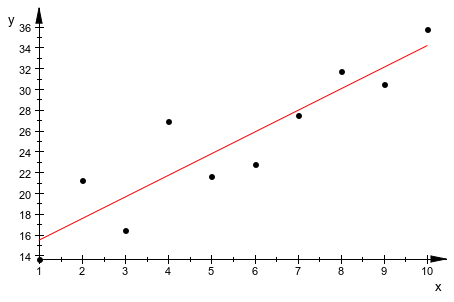
\includegraphics[width=10cm]{univariate-linear-regression} 
 	
	\item Explain about univariate non-linear regression.
	\par Univariate non-linear regression adalah salah satu jenis regresi di mana hanya terdapat satu variabel bebas, namun berbeda dengan regresi linear, pada regresi jenis ini, hubungan antara variabel dependent dan variabel independentnya (variable bebas) tidak linear. Selain itu, menurut [4], non-linear regression berarti \textit{'the regression function is not simultaneously linear in the unknown parameter $\beta_i$'}

	\par 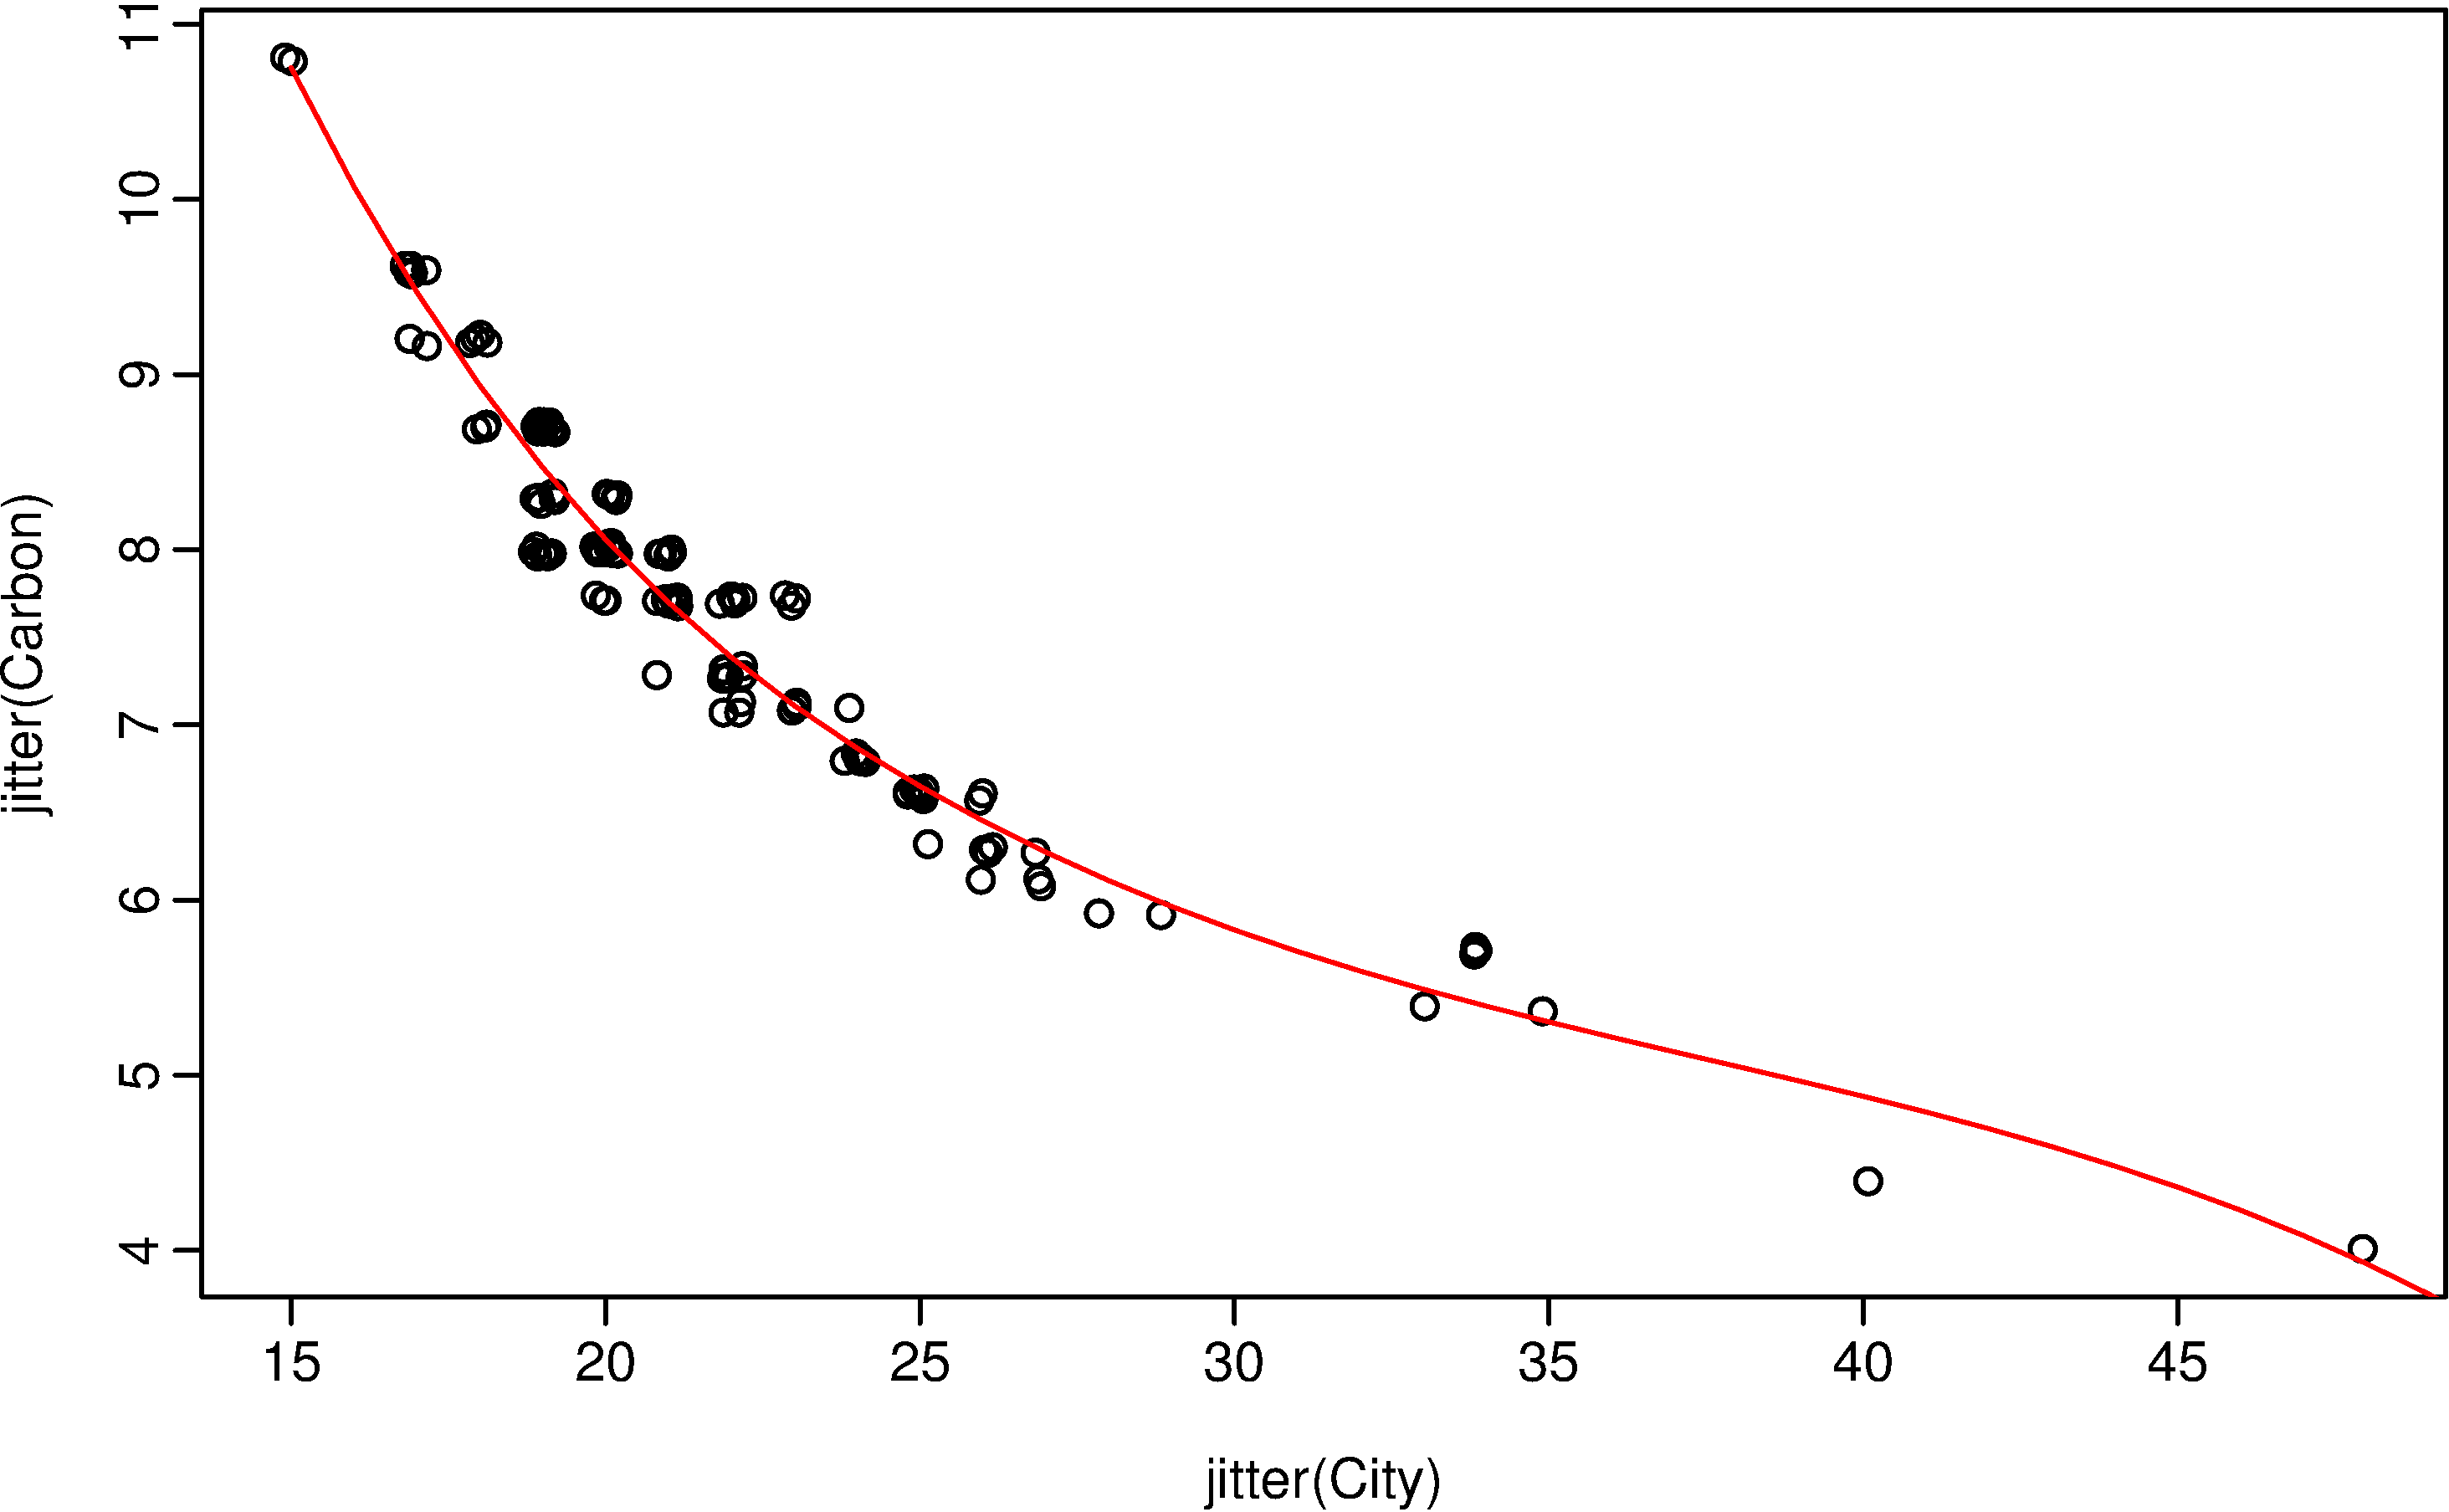
\includegraphics[width=10cm]{univariate-nonlinear-regression}

	\par Salah satu contoh model regresi ini adalah model Michaelis-Menten untuk kinetik enzim[3]

		\[v = \frac{V_{max} \left [ \textup{S} \right ]}{K_m + \left [ \textup{S} \right ]}\]

	\par yang dapat dituliskan menjadi

		\[f(x,\beta) = \frac{\beta_1 x}{\beta_2 + x}\]

	\par di mana $\beta_1$ adalah parameter $V_{max}$ , $\beta_2$ adalah parameter $ K_m $ dan $\left [ \textup{S} \right ]$ adalah variabel independent, $x$. Fungsi ini termasuk model non-linear karena fungsi ini tidak dapat diekspresikan sebagai kombinasi linear dari dua $\beta$. Contoh lain dari fungsi nonlinear adalah fungsi eksponensial, fungsi logaritmik, fungsi trigonomoteri, fungsi kuadrat, dan fungsi Gaussian[3].

	\item \textbf{(5 points)} Explain about multivariate linear regression 
	\par Multivariate linear regression adalah regresi linear yang variabel bebas yang terlibat tidak hanya satu, melainkan beberapa variabel bebas. [3] Karena input yang digunakan lebih dari satu dimensi, maka model regresi linear ini berbeda dengan model regresi linear univariat, yaitu

		\[h_w(x) = w_0 + w_1x_1 + w_2x_2 + \cdots + w_mx_m\]

		\[h_w(x) = w_0 + \sum_{i=0}^{m}w_ix_i\]

	\par di mana $w$ juga merupakan nilai yang akan dicari sedemikian sehingga nilai $w$ menjadi optimal dan $x$ merupakan variabel bebas atau input. Untuk mencari nilai $w$, kita dapat menggunakan cara yang sama dengan regresi linear univariat, yaitu dengan menggunakan metode \textit{least square}, \textit{maximum likehood}, atau algoritma \textit{gradient descent}.

	\par Selain itu, untuk mendefenisikan regresi linear multivariat, juga dapat menggunakan bentuk persamaan lain, menurut [5], yaitu

		\[y = X\omega + \epsilon\]

	\par di mana \textit{residual} (sisa) $\epsilon_i = y_i - \omega \cdot x_i$ mengindikasikan error yang dihasilkan oleh vektor berat $w$ pada titik $(x_i , y_i)$. Cara untuk menemukan besar $\omega$ adalah dengan meminimasikan \textit{sum of squared residual},

		\[\sum_{i=1}^{n} \epsilon_i^2 = \left \| \mathbf{\epsilon} \right \|^2_2\]


	\item \textbf{(5 points)} Explain about multivariate non-linear regression
	\par Multivariate non-linear regression adalah regresi linear yang melibatkan variabel bebas lebih dari satu (sama seperti regresi linear multivariate), namun berbeda dengan regresi linear multivariat, bidang hasilnya tidak linear (lurus).

	\par Menurut [5], kita dapat memodelkan fungsi nonlinear dengan membuat input matriksnya. Misal untuk 

		\[y_i = f(x_i) = \omega_0 + \omega_1x_{i1} + \omega_2x_{i2} + \omega_3x_{i3} + \omega_3x_{i1} x_{i2}\]

	\par kita membuatkan matrix inputnya mnejadi

		\[\textup{\textbf{X}} = \begin{pmatrix} 1 & x_{11} & x_{12} & x_{11}x_{12}\\ 1 & x_{21} & x_{22} & x_{21}x_{22}\\ 1 & x_{31} & x_{32} & x_{31}x_{13}\\ 1 & x_{41} & x_{42} & x_{41}x_{42}\\ \vdots & \vdots & \vdots & \vdots \end{pmatrix} , \textup{dan} \ \textup{\textbf{y}} = \begin{pmatrix} y_1\\ y_2\\ y_3\\ y_4\\ \vdots \end{pmatrix}\]

	\item \textbf{(5 points)} Explain the advantages of Multi-Layer Perceptron (MLP).
	\par MLP adalah algoritma yang sangat baik untuk digunanakan untuk regresi dan \textit{mapping}. Ia dapat digunakan untuk memetakan sinyal input dengan dimensi-N ke sinyal output dimensi-M, dan pemetaan ini juga bisa non-linear[6]

	\par Selain itu, MLP juga memiliki kemampuan untuk memodelkan relasi yang lebih kompleks antara input dan output[2] dengan akurasi yang tinggi[2] (akurasi juga bergantung pada fungsi aktivasi yang digunakan).

	\item \textbf{(5 points)} Explain the disadvantages of MLP.
	\par Karena memiliki beberapa perceptron, MLP memerlukan waktu \textit{training} yang lebih lama dan dilakukan berulang kali sampai jumlah tertentu untuk mendapatkan akurasi yang lebih baik, apalagi jika \textit{hidden-node atau hidden-layer}nya besar/banyak.

	\item \textbf{(5 points)} Explain the similarities between MLP and Support Vector Machine (SVM)
	\par Dalam mengklasifikasikan data, MLP dan SVM sama-sama mencari garis yang memisahkan data yang disebut \textit{decision-boundary}[2].

	\item \textbf{(5 points)} Explain the differences between MLP and SVM.
	\par Dalam menentukan \textit{decision-boundary}, MLP akan membuat \textit{decision-boundary} secara acak, kemudian seiring berjalannya learning, MLP akan mengupdate \textit{decision-boundary}-nya dengan mengupdate bias atau \textit{synaptic weight}-nya[2].

	\par Sedangkan SVM menggunakan perhitungan tertentu, bahkan akan memproses data terlebih dahulu menggunakan fungsi kernel (jika diperlukan atau jika data tidak dapat dipisahkan secara linear) untuk kemudian dipisahkan menggunakan \textit{decision-boundary} dengan \textit{learning rate} tertentu[2].

	\item \textbf{(5 points)} Describe the influences of number of neurons to the MLP model.
	\par Jumlah neuron dalam tiap \textit{layer} berbeda-beda. Pada \textit{input layer}, jumlah neuron harus sesuai dengan jumlah atribut yang akan diproses. Sedangkan pada \textit{hidden layer}, jumlah neuron $\geq 1$. Pada layer ini, jumlah neuron yang terbaik dicari dengan mencoba mengganti jumlah neuron (\texit{trial and error}). Yang terakhir, pada \textit{output layer}, jumlah neuron disesuaikan dengan banyaknya kelas.[2][7]

	\item \textbf{(5 points)} Describe the influences of type of activation function to the MLP model.
	\par Tanpa menggunakan fungsi aktivasi, \textit{ouput signalnya} adalah fungsi linear sederhana.[8] Selain itu, fungsi aktivasi penting untuk proses \textit{learning} dan digunakan untuk mengubah nilai \textit{input} menjadi nilai tertentu, yang kemudian digunakan untuk mengaktifkan atau menonaktifkan neuron.[2]

	\par Pemilihan fungsi aktivasi bisa dengan cara mencoba sesuai kebutuhan. namun dari beberapa literatur, untuk \textit{hidden layer}, sebaiknya menggunakan ReLu. Dan jika ternyata model kita memiliki banyak \textit{dead neuron} selama proses \textit{training}, maka sebaiknya kita menggunakan fungsi ReLu atau Maxout.


	\item \textbf{(5 points)} Describe the influences of learning rate to the MLP model.
	\par Pada MLP, \textit{learning rate} memiliki pengaruh pada perubahan \textit{decision-boundary}. Semakin besar nilai \textit{learning rate} maka semakin besar perubahan \textit{decision-boundary} dan sebaliknya. \textit{Learning rate} yang kecil, mengakibatkan sebuah model membutuhkan proses \textit{learning} yang lebih banyak atau epoch yang lebih banyak, untuk mendapatkan \textit{decision-boundary} yang optimal. Sedangkan \textit{learning rate} yang besar, mengakibatkan \textit{decision-boundary} sulit atau bahkan tidak dapat mencapai titik optimal.

	\item \textbf{(5 points)} Explain how MLP obtains optimal decision boundary.
	\par Untuk mendapatkan \textit{decision-boundary} yang optimal, akan memproses inputan hingga mendapatkan \textit{error}, dengan menentukan nilai bobot random dna memrposesnya hingga \textit{layer} output. Kemudian, nilai \textit{error} tersebut diproses lagi ke \textit{layer input} dengan arah terbalik. Hasil dari proses ini kemudian digunakan untuk mengupdate nilai bobot yang akan diproses lagi. Langkah bolak-balik atau maju-mundur ini akan dilakukan berulang-ulang hingga nilai \textit{error} tertentu atau sebanyak epoch yang telah ditentukan. Nilai akhir atau nilai bobot yang telah di-\textit{update} akan membantu mempengaruhi MLP dalam membentuk \textit{decision-boundary} yang optimal.


	\item \textbf{(5 points)} Explain how SVM obtains optimal hyperplane.
	\par Untuk mendapatkan hyperplane yang optimal, SVM harus memaksimalkan \textit{decision-boundary} atau dengan hyperplane dengan margin paling besar (yang membuat SVM sering disebut \textit{maximal margin classifier}) [2].
	\par Misal dalam \textit{binary classification} yang terdiri dari contoh \textit{training} sebanyak $N$. Setiap contoh dinotasikan oleh \textit{tuple} $(\textbf{x}_i,y_i)(i = 1,2,...,N)$, dimana $\textbf{x}_i = (x_{i1},x_{i2},...,x_{id})^T$ berhubungan dengan set atribut contoh ke-i, $y_i \in \left \{ -1 , 1 \right \}$ sebagai label kelasnya. \textit{Decision-boundary} dari sebuah \textit{linear classifier} dapat ditulis dalam bentuk[2]

	\[\textup{\textbf{w}} \cdot \textup{\textbf{x}} + b = 0\]

	\par di mana $\textup{\textbf{w}}$ dan $b$ adalah parameter dari model. Untuk memaksimalkan \textit{margin}-nya, sama dengan meminimalkan \textit{objective function} berikut[2]

	\[f(\textup{\textbf{w}} ) = \frac{\left \| \textup{\textbf{w}} \right \|^2}{2}\]

	\par Namun, fungsi objektif ini bersifat kuadratik dan \textit{constraints}-nya linear dalam parameter $\textup{\textbf{w}}$ dan $b$, yang dikenal sebagai \textit{convex optimization problem}, yang dapat diselesaikan menggunakan metode \textit{Lagrange Multiplier}.

	\par Fungsi objektif yang kemudian digunakan sesuai masalah, \textit{Langrangian} untuk optimisasi:

	\[L_P = \frac{1}{2}\left \| \textup{\textbf{w}} \right \|^2 - \sum_{i=1}^{N}\lambda_i\left ( y_i\left ( \textup{\textbf{w}} \cdot \textup{\textbf{x}}_i + b \right ) -1 \right )\]

	\par Kemudian untuk meminimasikan \textit{Langrarian}, kita harus menggunakan turunan $L_p$ terhadap $\textup{\textbf{w}}$ dan $b$ dan menjadikannya 0 :

	\[\frac{\partial Lp }{\partial\textup{\textbf{w}}} = 0 \Rightarrow \textup{\textbf{w}} = \sum_{i=1}^{N} \lambda_i y_i \textup{\textbf{x}}_i\]

	\[\frac{\partial Lp }{\partial\textup{\textbf{b}}} = 0 \Rightarrow \textup{\textbf{w}} = \sum_{i=1}^{N} \lambda_i y_i = 0\]
 
	\par Namun, karena pengali dari \textit{Langrage} tidak diketahui, maka kita tidak dapat mencari $\textup{\textbf{w}}$ dan $b$. Untuk itu, perlu dilakukan transformasi pada pengali \textit{Langrage}, yang diketahui sebagai kondisi Karush-Kuhn-Tucker : 

		\[\lambda_i \geq 0\]
		\[\lambda_i \left [ y_i(\textup{\textbf{w}} \cdot \textup{\textbf{x}}_i + b) -1 \right ] = 0\]

	\par yang kemudian mengarah ke

		\[L_D = \sum_{i=1}^{N} \lambda_i - \frac{1}{2} \sum_{i,j} \lambda_i \lambda_j y_i y_j \textup{\textbf{x}}_i \cdot \textup{\textbf{x}}_j\]

	\par Kemudian, \textit{decision-boundary}-nya dapat diekspresikan menggunakan [2]

		\[\left ( \sum_{i=1}^{N} \lambda_i y_i\textup{\textbf{x}}_i \cdot \textup{\textbf{x}} \right ) + b = 0\]

	\item \textbf{(5 points)} Explain how SVM classifies data sets that are non-linearly separable.
	\par Untuk mengklasifikasikan data yang \textit{non-linearly separable}, SVM menggunakan fungsi kernel untuk memetakan data ke bidang baru yang memungkinkan SVM untuk membuat garis pemisah.

	\par Contoh dampak transformasi pemetaan data pada bidang koordinat $\textup{\textbf{x}}$ ke bidang koordinat $\Phi (\textup{\textbf{x}})$, yang membuat data dapat dipisahkan secara linear, dapat dilihat pada gambar berikut:

	\par 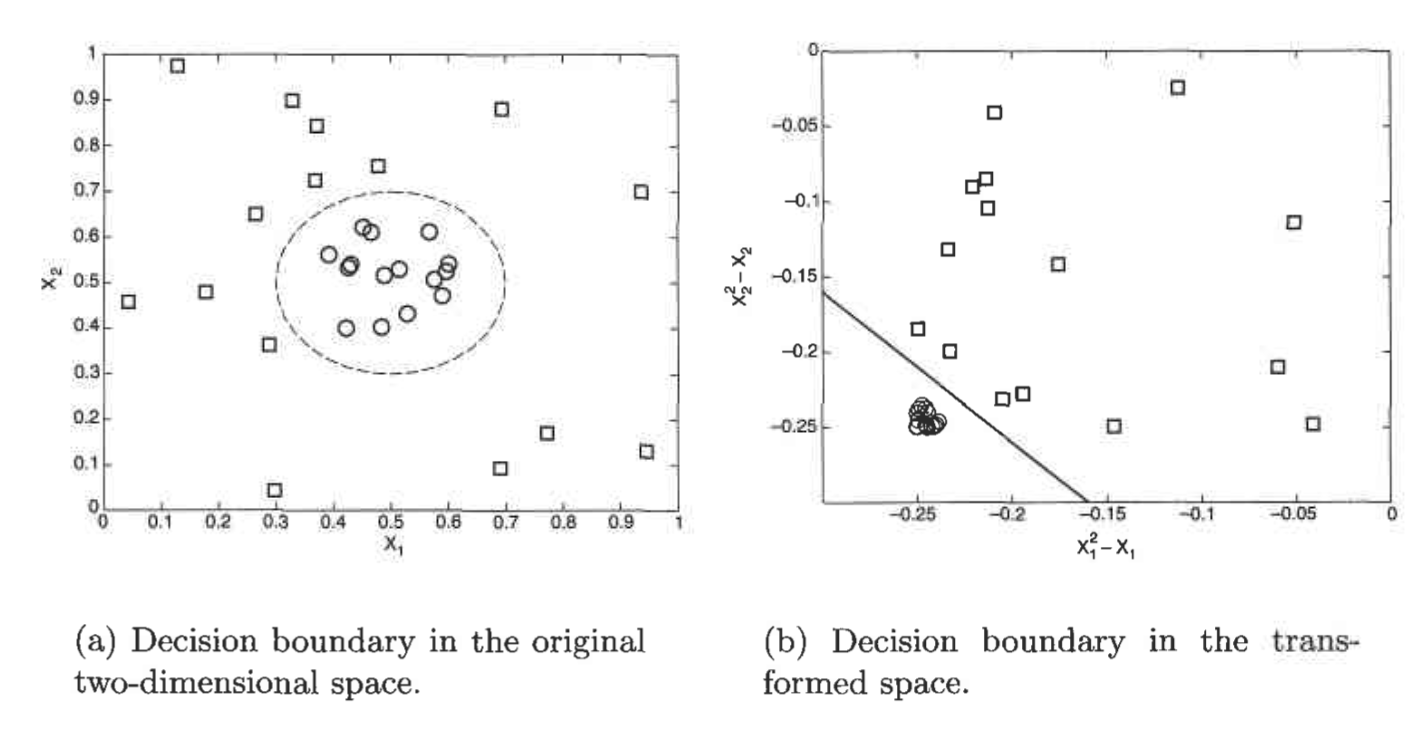
\includegraphics[width=10cm]{svm-transform} 

\end{enumerate}

\par \textbf{Referensi}
\par [1] https://id.wikipedia.org/wiki/Regresi_Linier
\par [2] Introduction to Data Mining - Panning Tan, M. Steinbach
\par [3] https://en.wikipedia.org/wiki/Nonlinear_regression
\par [4] Regression book
\par [5] Regression slide
\par [6] http://www.nickgillian.com/wiki/pmwiki.php/GRT/MLP
\par [7] Machine Learning - Tom Mitchell
\par [8] https://medium.com/towards-data-science/activation-functions-and-its-types-which-is-better-a9a5310cc8f
\par [9] Slide ANN-MLP Machine Learning

\end{document}

